One of the simplest parallel sorting algorithms is odd-even sort also know as odd-even transposition sort and brick sort. It is a comparison sort and can be seen as the parallel version of the simple serial bubble sort. The odd-even sort consists of two phases a odd and an even. In each phase each odd or even index array pair is compared and swapped if necessary. An visual representation of the odd-even sort is seen in \cref{fig:sort_odd_even}.

\begin{figure}[ht]
	\centering
	\fbox{
		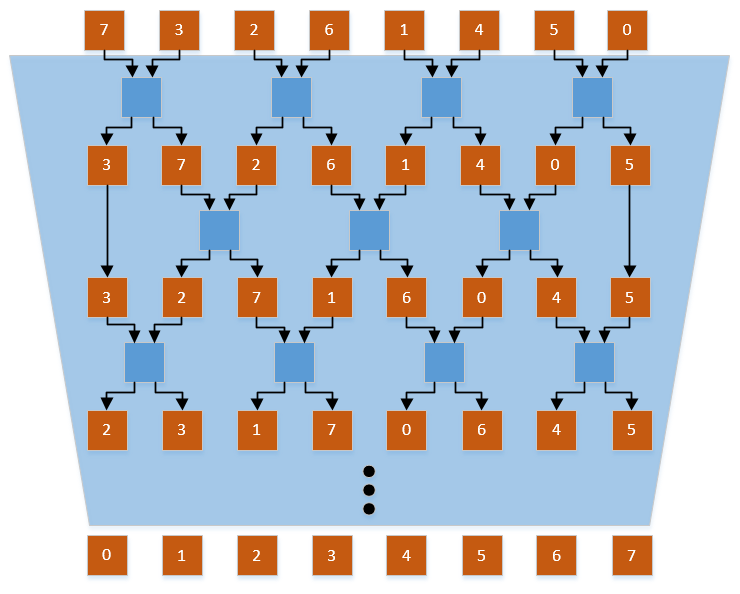
\includegraphics[width=0.5\textwidth]{figs/algorithm/sort_odd_even.png}}
	\caption{Odd-even sort, orange blocks are data elements, and blue blocks are compare-and-swap operations}
	\label{fig:sort_odd_even}
\end{figure}  

The odd-even sort have a worst-case step complexity of $\mathcal{O}(n)$ as the maximum number of array position an element can move is $n$. The worst case work complexity is $\mathcal{O}(n^2)$ as $\mathcal{O}(n)$ operations is carried out in $\mathcal{O}(n)$ steps. The odd-even sort is step efficient when compared to serial versions, but other parallel sorting algorithms are more efficient.   